\subsection{波莱尔集}

定义 3. 设 X 是一个集，\(\mathfrak{X}\) 是 X 的子集所成的一个集。\(\mathfrak{X}\) 称为 X 上的一个 \(\sigma\) 代数，如果下列条件满足：

\begin{enumerate}
\def\labelenumi{\alph{enumi})}
\item
  \(\mathfrak{S}\) 中每个集的余集属于 \(\mathfrak{S}\) 。
\item
  \(\mathfrak{X}\) 中集合的每个可数交属于 \(\mathfrak{X}\) 。
\end{enumerate}

若 \(\mathfrak{X}\) 是一个 \(\sigma\) 代数（在 \(\mathbf{X}\) 上），则 \(\mathfrak{X}\) 中集合的每个可数并都属于 \(\mathfrak{X}\) （因为此并的余集是 \(\mathfrak{X}\) 中集合的交）。

X 的所有子集所成的集 \(\mathfrak{P}(\mathbf{X})\) 显然是一个 \(\sigma\) 代数。X 上的 \(\sigma\) 代数的每个交是 X 上的 \(\sigma\) 代数。因此，对 \(\mathfrak{P}(\mathbf{X})\) 的任意子集 F ，存在包含 F 的最小 \(\sigma\) 代数；它称为由 F 生成的 \(\sigma\) 代数。

定义 4. 在拓扑空间 X 中，由 X 的所有闭子集所成的集生成的 \(\sigma\) 代数的元素称为 X 中的波莱尔集。

命题 10. 设 \(f\) 是拓扑空间 \(\mathbf{X}\) 到拓扑空间 \(\mathbf{Y}\) 中的连续映射。则在 \(f\) 之下，\(\mathbf{Y}\) 中每个波莱尔集的原像是 \(\mathbf{X}\) 中的波莱尔集。

设 \(\mathfrak{X}\) 是满足如下条件的诸集 \(\mathbf{A}\) （ \(\mathbf{Y}\) 的子集）所成的集：\(\overline{f}^1 (\mathbf{A})\) 是 \(\mathbf{X}\) 中的波莱尔集。由此立得 \(\mathfrak{X}\) 是一个 \(\sigma\) 代数，它包含 \(\mathbf{Y}\) 的所有闭子集；从而 \(\mathfrak{X}\) 包含 \(\mathbf{Y}\) 中的所有波莱尔集。

命题 11. 在苏斯林空间 X 中，每个波莱尔集都是苏斯林集。

设 \(\mathfrak{X}\) 是由 X 的诸子集 A 中 A 与 CA 都是苏斯林集者所成的集。由第 2 号的命题 8 ，\(\mathfrak{X}\) 是一个 \(\sigma\) 代数。X 的每个闭子集 F 属于 \(\mathfrak{X}\) ，因为 F 与 CF 都是苏斯林集（第 2 号，命题 5）；从而 \(\mathfrak{X}\) 包含 X 的所有波莱尔集（参看第 6 号，定理 2 的推论）。

推论. 设 \(f\) 是苏斯林空间 \(\mathbf{X}\) 到可度量化空间 \(\mathbf{Y}\) 中的连续映射。若 \(\mathbf{B}\) 是 \(\mathbf{X}\) 中的任意波莱尔集，则 \(f(\mathbf{B})\) 是 \(\mathbf{Y}\) 中的苏斯林集。

因为 B 是苏斯林空间，故由定义 2 后的注（第 2 号），\(f(\mathbf{B})\) 也是苏斯林空间。

\pandocbounded{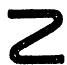
\includegraphics[keepaspectratio]{images/part002_bde2d1b5.jpg}}

注。1) 即使 X 与 Y 都是波兰空间，一般说来，X 中的波莱尔集在 X 到 Y 中的连续映射下的像未必是 Y 中的波莱尔集（参看习题 6；以及第 7 号，定理 3 的推论）。

\begin{enumerate}
\def\labelenumi{\arabic{enumi})}
\setcounter{enumi}{1}
\tightlist
\item
  设 X 是拓扑空间，Y 是 X 的波莱尔子集。则空间 Y 的波莱尔集恰是 X 的含于 Y 的那些波莱尔集。因为 (i) X 中含于 Y 的波莱尔集构成 Y 上的一个 σ 代数，它包含 Y 中的闭集，从而包含 Y 的所有波莱尔集；(ii) X 的使 A∩Y 是 Y 的波莱尔集的那些子集 A 构成 X 上的一个 σ 代数，它包含 X 的所有闭集，从而包含 X 的所有波莱尔集。
\end{enumerate}

